In this project, we will investigate numerical methods which may be
amenable to quantum computing, once converted to an appropriate form
and simulated on a quantum device.  To this end we have discussed
several potential methods that could take advantage of the design of a
quantum computer, two of which are described below:
\begin{itemize}
\item \emph{High-Dimensional Numerical Integration}: Approximation of
  integrals defined in many spatial dimensions and/or over complex
  domains; tradiationally relying on ``Monte Carlo'' integration
  algorithms.
\item \emph{Derivative-Free Optimization}: minimization of complex
  functionals that depend non-differentiably a set of variables, for
  which tradiational gradient-based information is unavailable.  These
  often rely on statistical opimization approaches including ``genetic
  optimization'' and ``simulated annealing''.
\end{itemize}
This problem of constructing numerical algorithms that may utilize
quantum computing is extremely practical as we are entering the age of
``big data,'' where more efficient numerical methods need to be
explored in order to balance increasing data set sizes.  

We also plan to take advantage of previous work in the realm of
quantum summation and integration \cite{Traub:2002}. Although we will
make use of these quantum algorithms in our research, the real utility
of this project is presented in the next section, where we will
discuss our previous work in this area.

    %\begin{figure} [h!]
      %  \centering
     %   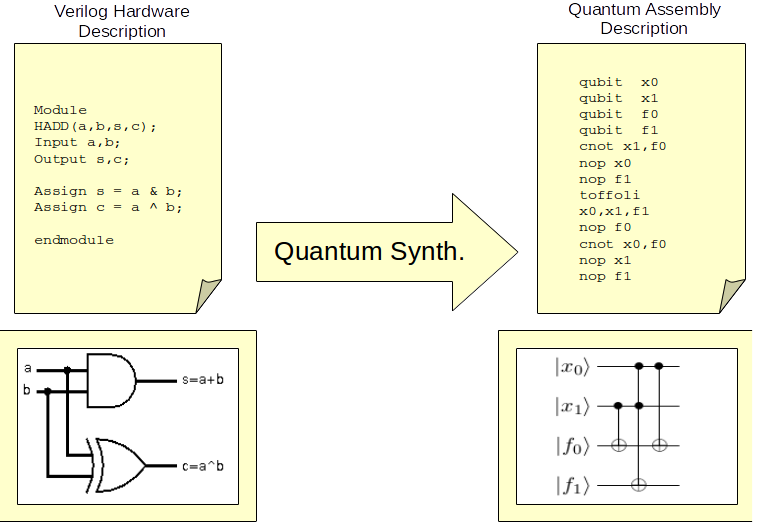
\includegraphics[scale = 0.35]{QuantumSynthesis.png}
    %\end{figure}

